% \pagebreak[4]
% \hspace*{1cm}
% \pagebreak[4]
% \hspace*{1cm}
% \pagebreak[4]

\chapter{Mở đầu}
\textit{Nội dung của chương 1 giới thiệu tổng quan về đề tài, nêu ra mục tiêu của khóa luận, và cấu trúc nội dung của luận văn.}
\ifpdf
    \graphicspath{{Chapter1/Chapter1Figs/PNG/}{Chapter1/Chapter1Figs/PDF/}{Chapter1/Chapter1Figs/}}
\else
    \graphicspath{{Chapter1/Chapter1Figs/EPS/}{Chapter1/Chapter1Figs/}}
\fi

\section{Tổng quan về đề tài}

\subsection{Giới thiệu về trợ lý ảo}

Trợ lý ảo là một phần mềm trên máy tính hoặc thiết bị di động có khả năng hỗ trợ người dùng thực hiện nhiều loại công việc, nhận lệnh từ người dùng dưới dạng ngôn ngữ tự nhiên, thường là giọng nói. Nhờ khả năng nhận lệnh và phản hồi qua giọng nói, người dùng có thể ra lệnh cho trợ lý ảo mà không cần phải thao tác bằng tay trên thiết bị. Điều đó sẽ giúp tăng tính hiệu quả và tạo ra sự tự nhiên trong giao tiếp giữa người và máy, tạo ra những kênh tương tác mới khác với truyền thống, mang đến cho người dùng những trải nghiệm mới mẻ và thứ vị hơn khi sử dụng những thiết bị công nghệ.

Chức năng của các trợ lý ảo rất phong phú và đa dạng, từ những chức năng bình thường như hỏi đáp, tra cứu thông tin, bật nhạc, tìm kiếm trong danh bạ, quản lý lịch, đặt báo thức,... cho đến những chức năng đặc biệt như chơi game, trò chuyện, điều khiển các thiết bị trong gia đình, thậm chí là mua sắm, đặt chỗ nhà hàng, đặt vé máy bay,...

\subsection{Khảo sát thị trường trợ lý ảo}

Tính đến hiện tại, gần như tất cả các hãng công nghệ lớn đều đã tung ra trợ lý ảo của riêng mình:

\begin{itemize}
    \item Apple với Siri, hoạt động trên các thiết bị của Apple như iPhone, iPad, iPod Touch, Mac và Apple TV.
    \item Microsoft với Cortana, hoạt động trên các phiên bản mới của Windows như Windows 10, Windows 10 Mobile, Windows Phone 8.1, và các thiết bị khác như Microsoft Band, Xbox One.
    \item Amazon với Alexa, hoạt động trên loa thông minh Amazon Echo.
    \item Google với Google Assistant, hoạt động trên các thiết bị Android, loa thông minh Google Home và ứng dụng nhắn tin Allo.
    \item Gần đây, Samsung đã ra mắt trợ lý ảo của mình mang tên Bixby, chạy trên các dòng điện thoại Samsung Galaxy.
    \item Facebook cũng đã công bố trợ lý ảo của mình mang tên M, sẽ ra mắt trong năm 2017 trên các ứng dụng Facebook và Facebook Messenger.
\end{itemize}

Trong xu hướng đó, số lượng người dùng và tần suất sử dụng của các trợ lý ảo đang ngày càng gia tăng. Theo một khảo sát thực hiện vào tháng 01/2017 trên các người dùng smartphone tại Mỹ\cite{emarketerreport}, có gần 27\% người được hỏi nói rằng họ dùng trợ lý ảo ít nhất một lần mỗi tuần, và khoảng 22\% người dùng sử dụng trợ lý ảo hàng ngày. Trong khi đó, có 28.7\% số người được hỏi chưa bao giờ sử dụng trợ lý ảo.

\begin{figure}[h]
    \centering
    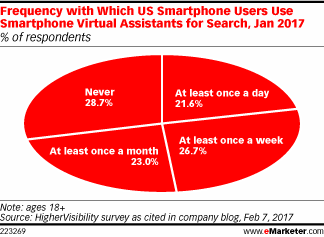
\includegraphics[scale=1]{emarketer_1}
    \caption[Tần suất người dùng smartphone ở Mỹ sử dụng trợ lý ảo]{Tần suất người dùng smartphone ở Mỹ sử dụng trợ lý ảo, tháng 01/2017\cite{emarketerreport}}
    \label{fig:c1_emarketer_1}
\end{figure}

Khi được hỏi về lý do sử dụng trợ lý ảo, 1/3 số người được hỏi nói rằng tìm kiếm bằng trợ lý ảo dễ hơn tìm kiếm bằng tay. Khoảng 1/4 số người được khảo sát nói rằng họ không thể gõ chữ trên smartphone, hoặc không thể nhìn rõ trên smartphone, hoặc vì tìm kiếm bằng trợ lý ảo nhanh hơn tìm kiếm bằng tay. Tuy nhiên, lý do lớn nhất mà nhiều người dùng sử dụng trợ lý ảo là lái xe. Có đến hơn một nửa số người được hỏi cho biết họ sử dụng trợ lý ảo trong khi lái xe.

\begin{figure}[h]
    \centering
    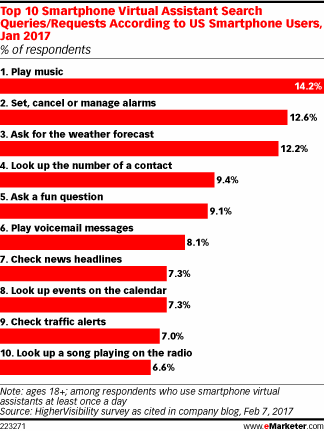
\includegraphics[scale=1]{emarketer_2}
    \caption[Những chức năng được sử dụng nhiều nhất trên trợ lý ảo]{Những chức năng được sử dụng nhiều nhất trên trợ lý ảo theo người dùng smartphone ở Mỹ, tháng 01/2017\cite{emarketerreport}}
    \label{fig:c1_emarketer_2}
\end{figure}

Nhìn vào hình \ref{fig:c1_emarketer_2} có thể thấy phần đông người dùng sử dụng trợ lý ảo với mục đích bật nhạc, quản lý báo thức, hỏi thông tin dự báo thời tiết. Ngoài ra, họ còn dùng trợ lý ảo để tìm kiếm số điện thoại trong danh bạ, hỏi câu hỏi vui, bật các tin nhắn thoại hoặc xem tin tức.

Như vậy có thể nói các trợ lý ảo đang ngày càng góp một phần quan trọng trong cuộc sống của những người dùng công nghệ. Không chỉ tạo ra một trải nghiệm mới, các trợ lý ảo còn giúp tiết kiệm thời gian và công sức. Ngoài ra, các trợ lý ảo còn có thể giúp được những người khuyết tật hoặc người cao tuổi có thể tiếp cận với các thiết bị công nghệ một cách dễ dàng hơn.

\section{Mục tiêu của khóa luận}

Nhận thấy các trợ lý ảo nêu trong phần trước đa phần chỉ hoạt động trên một số nền tảng nhất định của hãng làm ra chúng, và chủ yếu dành cho các thiết bị di động, chúng tôi thực hiện khóa luận này với mục đích chính là tạo ra một ứng dụng trợ lý ảo có khả năng chạy trên các nền tảng hệ điều hành phổ biến trên máy tính cả nhân như Windows, Linux, Mac, với các chứng năng cơ bản:

\begin{itemize}
    \item Hỏi đáp, tra cứu thông tin
    \item Hỏi giờ, thời tiết
    \item Phát nhạc
    \item Trò chuyện đơn giản
\end{itemize}

Các mục tiêu nhỏ:

\begin{itemize}
    \item Ứng dụng có khả năng tự kích hoạt khi người dùng gọi tên
    \item Nhận biết chính xác câu nói của người dùng
    \item Phản hồi một cách chính xác và tự nhiên
    \item Thời gian xử lý ngắn (tính từ lúc người dùng hoàn thành câu nói đến lúc ứng dụng bắt đầu phản hồi).
\end{itemize}

\section{Nội dung luận văn}

Nội dung của luận văn sẽ gồm những phần sau:

\begin{itemize}
    \item Chương 1: \emph{Mở đầu}: Giới thiệu tổng quan về đề tài, mục tiêu của khóa luận và cấu trúc nội dung của luận văn.
    \item Chương 2: \emph{Tổng quan về tín hiệu âm thanh, tiếng nói. Thư viện PyAudio}: Giới thiệu tổng quan về tín hiệu âm thanh, tiếng nói, các thành phần của âm thanh, cách lưu trữ âm thanh trong máy tính, các thông số của file âm thanh; giới thiệu về thư viện PyAudio: chức năng, cách cài đặt, cách sử dụng.
    \item Chương 3: \emph{Speech to Text}: Giới thiệu về bài toán Speech to Text, các ứng dụng, các vấn đề cần giải quyết trong Speech to Text; giới thiệu về các thư viện pocketsphinx và Google Speech to Text: chức năng, cách cài đặt, cách sử dụng, ưu và nhược điểm, vai trò của các thư viện đó trong hệ thống.
    \item Chương 4: \emph{Text to Speech}: Giới thiệu về bài toán Text to Speech, các ứng dụng; giới thiệu về Google Text to Speech và iSpeech: chức năng, cách sử dụng, ưu và nhược điểm, vai trò trong hệ thống.
    \item Chương 5: \emph{Intent Classification}: Giới thiệu về bài toán Intent Classification, các thuật toán để giải quyết bài toán này, các ứng dụng; giới thiệu về thư viện Rasa NLU: chức năng, cách cài đặt, cách sử dụng, vai trò trong hệ thống.
    \item Chương 6: \emph{Ứng dụng Alexa}: Giới thiệu tổng quan về ứng dụng Alexa, các module trong chương trình, luồng hoạt động giữa các module, các chức năng của ứng dụng.
    \item Chương 7: \emph{Kết luận và Hướng phát triển}: Nếu ra các kết quả đạt được của khóa luận, các hạn chế và hướng phát triển.
\end{itemize}

